\documentclass[12pt]{article}
\usepackage[utf8]{inputenc}
\usepackage{amsmath, amssymb}
\usepackage{geometry}
\usepackage{tikz}
\usepackage{pgfplots}
\usepackage{xcolor}
\usepackage{adjustbox}
\usepackage{caption}

\geometry{a4paper, margin=1in}
\pgfplotsset{compat=1.18}

% --- Colors ---
\definecolor{DeepNavy}{HTML}{2E4057}
\definecolor{Teal}{HTML}{048A81}
\definecolor{WarmOrange}{HTML}{E85D04}
\definecolor{Gold}{HTML}{D4A03A}
\definecolor{DeepRed}{HTML}{D62828}
\definecolor{LightGray}{HTML}{F0F0F0}

\usetikzlibrary{shapes.geometric, arrows.meta, positioning, calc, backgrounds, decorations.pathreplacing}

\title{\bfseries A Visual Guide to Granular Instrumental Variables (GIV)}
\author{Intuition for Visual Learners}
\date{}

\begin{document}

\maketitle

\section{The Anatomy of a Firm Shock}
For a visual learner, the demand equation $y_{it} = \phi^d p_t + \eta_t + u_{it}$ is a hierarchy of influences. 

\begin{center}
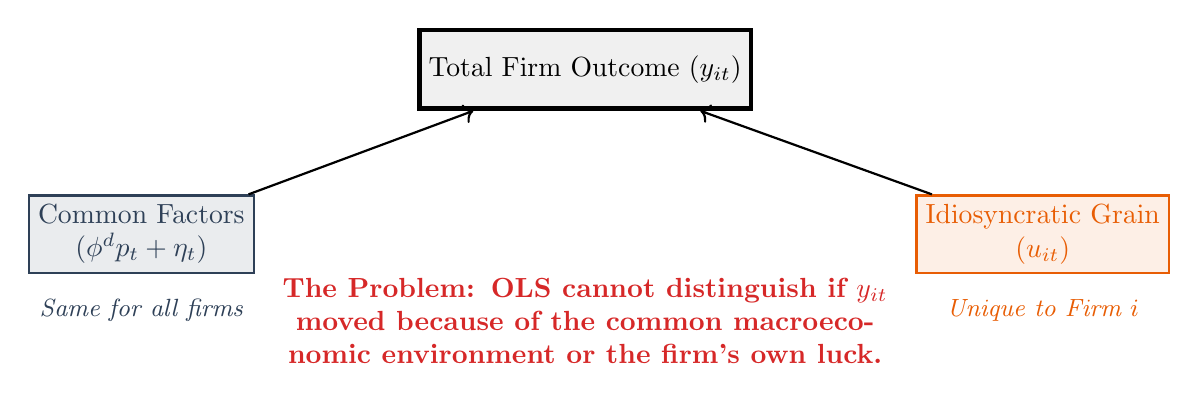
\begin{tikzpicture}[node distance=1.5cm, align=center]
    % Components
    \node (total) [draw, ultra thick, minimum width=4cm, minimum height=1cm, fill=LightGray] {Total Firm Outcome ($y_{it}$)};
    
    \node (common) [draw, DeepNavy, thick, below left=of total, xshift=-1cm, fill=DeepNavy!10] {Common Factors\\($\phi^d p_t + \eta_t$)};
    \node (idiosyncratic) [draw, WarmOrange, thick, below right=of total, xshift=1cm, fill=WarmOrange!10] {Idiosyncratic Grain\\($u_{it}$)};
    
    \draw[->, thick] (common) -- (total);
    \draw[->, thick] (idiosyncratic) -- (total);
    
    % The "Signal" vs "Noise"
    \node[below=0.2cm of common, font=\small\itshape, text=DeepNavy] {Same for all firms};
    \node[below=0.2cm of idiosyncratic, font=\small\itshape, text=WarmOrange] {Unique to Firm $i$};
    
    % The Problem
    \node[below=2cm of total, text=DeepRed, font=\bfseries, text width=10cm] {The Problem: OLS cannot distinguish if $y_{it}$ moved because of the common macroeconomic environment or the firm's own luck.};
\end{tikzpicture}
\end{center}

\section{The "Differencing" Mechanism}
The GIV ($z_t = y_{St} - y_{Et}$) is a filter. Imagine two "containers" of shocks. One is weighted by size (dominated by giants), and one is weighted equally (dominated by the crowd).

\begin{center}
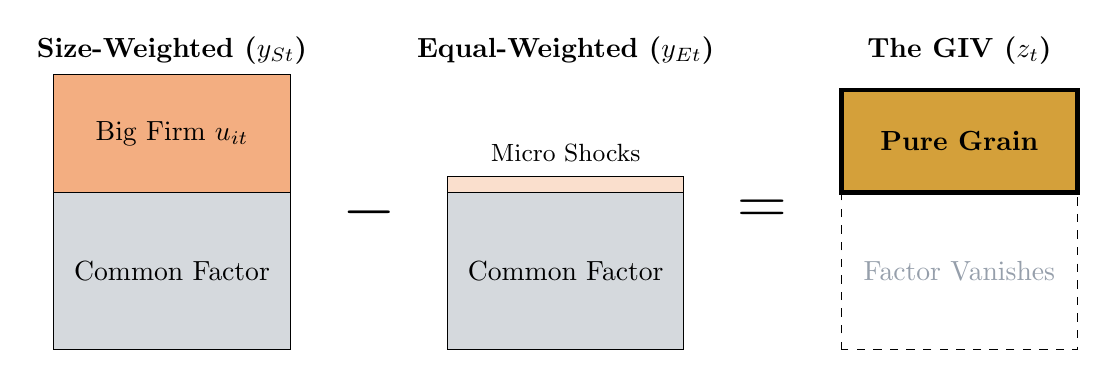
\begin{tikzpicture}
    % Size Weighted
    \begin{scope}[shift={(0,0)}]
        \node[above] at (1.5, 3.5) {\bfseries Size-Weighted ($y_{St}$)};
        \draw[fill=DeepNavy!20] (0,0) rectangle (3,2); % Common
        \draw[fill=WarmOrange!50] (0,2) rectangle (3,3.5); % Big firm shock
        \node at (1.5, 1) {Common Factor};
        \node at (1.5, 2.75) {Big Firm $u_{it}$};
    \end{scope}

    \node at (4, 1.75) {\Huge $-$};

    % Equal Weighted
    \begin{scope}[shift={(5,0)}]
        \node[above] at (1.5, 3.5) {\bfseries Equal-Weighted ($y_{Et}$)};
        \draw[fill=DeepNavy!20] (0,0) rectangle (3,2); % Common
        \draw[fill=WarmOrange!20] (0,2) rectangle (3,2.2); % Average tiny shocks
        \node at (1.5, 1) {Common Factor};
        \node at (1.5, 2.5) {\small Micro Shocks};
    \end{scope}

    \node at (9, 1.75) {\Huge $=$};

    % The GIV
    \begin{scope}[shift={(10,0)}]
        \node[above] at (1.5, 3.5) {\bfseries The GIV ($z_t$)};
        \draw[dashed] (0,0) rectangle (3,2); % Vanished common
        \draw[fill=Gold, ultra thick] (0,2) rectangle (3,3.3); % Pure grain
        \node[text=DeepNavy!50] at (1.5, 1) {Factor Vanishes};
        \node at (1.5, 2.65) {\bfseries Pure Grain};
    \end{scope}
\end{tikzpicture}
\end{center}

\newpage

\section{Why Granularity Matters (The Power Law)}
GIV only works if the "Big Firm Shock" in the previous diagram is large enough to survive the averaging. In a "Normal" economy (left), the GIV is just noise. In a "Granular" economy (right), the giants move the needle.

\begin{center}
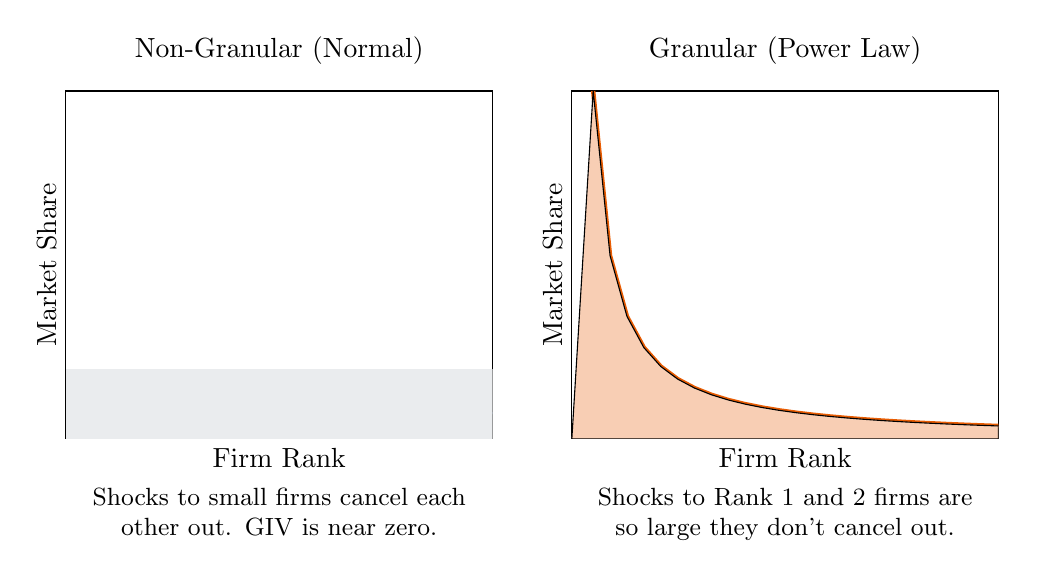
\begin{tikzpicture}
    \begin{axis}[
        name=normal,
        width=7cm, height=6cm,
        title={Non-Granular (Normal)},
        xlabel={Firm Rank}, ylabel={Market Share},
        xmin=0, xmax=20, ymin=0, ymax=1,
        ticks=none
    ]
        \addplot[DeepNavy, thick, domain=1:20] {0.2 * exp(-0.05*x)};
        \fill[DeepNavy!10] (axis cs:0,0) rectangle (axis cs:20,0.2);
    \end{axis}

    \begin{axis}[
        name=granular,
        at={($(normal.right of south east)+(1cm,0)$)},
        anchor=south west,
        width=7cm, height=6cm,
        title={Granular (Power Law)},
        xlabel={Firm Rank}, ylabel={Market Share},
        xmin=0, xmax=20, ymin=0, ymax=1,
        ticks=none
    ]
        \addplot[WarmOrange, ultra thick, domain=1:20] {1/x^1.1};
        \draw[fill=WarmOrange!30] (axis cs:0,0) -- plot[domain=1:20] (axis cs:\x,{1/\x^1.1}) -- (axis cs:20,0) -- cycle;
    \end{axis}
    
    \node[below=0.5cm of normal, text width=6cm, align=center, font=\small] {Shocks to small firms cancel each other out. GIV is near zero.};
    \node[below=0.5cm of granular, text width=6cm, align=center, font=\small] {Shocks to Rank 1 and 2 firms are so large they don't cancel out.};
\end{tikzpicture}
\end{center}

\section{Conceptual Flow of Identification}
How does $z_t$ help us find the causal effect $\psi$? 

\begin{center}
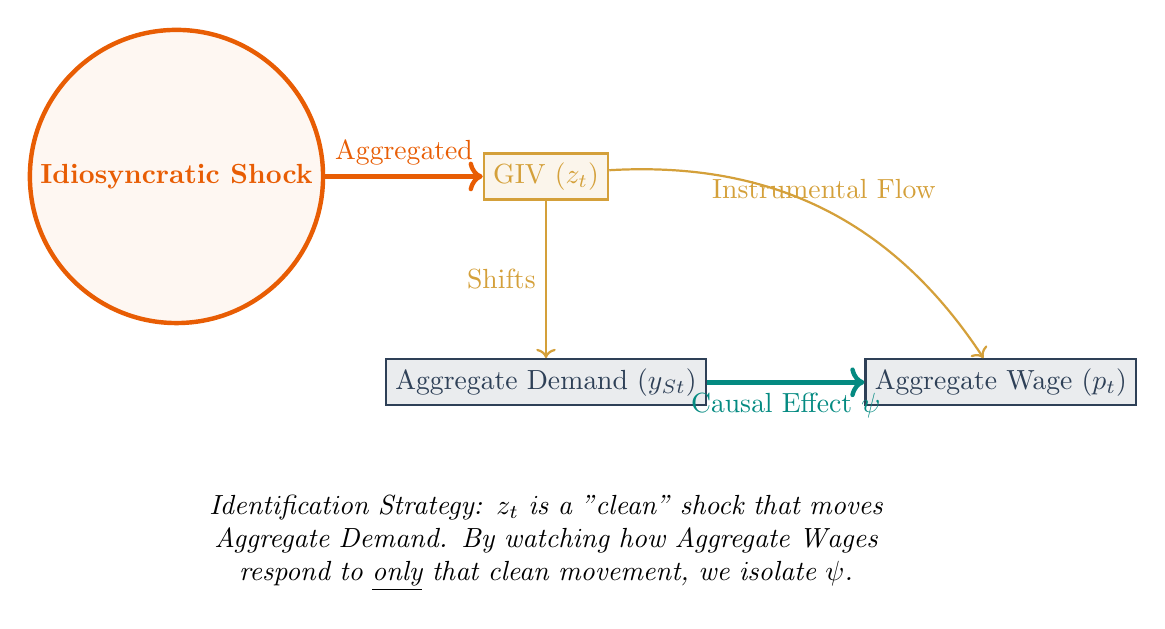
\begin{tikzpicture}[node distance=2cm, auto]
    \node (shock) [circle, draw, WarmOrange, ultra thick, fill=WarmOrange!5] {\bfseries Idiosyncratic Shock};
    \node (giv) [rectangle, draw, Gold, thick, right=of shock, fill=Gold!10] {GIV ($z_t$)};
    \node (aggregate) [rectangle, draw, DeepNavy, thick, below=of giv, fill=DeepNavy!10] {Aggregate Demand ($y_{St}$)};
    \node (price) [rectangle, draw, DeepNavy, thick, right=of aggregate, fill=DeepNavy!10] {Aggregate Wage ($p_t$)};
    
    \draw[->, ultra thick, WarmOrange] (shock) -- (giv) node[midway, above] {Aggregated};
    \draw[->, thick, Gold] (giv) -- (aggregate) node[midway, left] {Shifts};
    \draw[->, thick, Gold] (giv) to [bend left] node[above] {Instrumental Flow} (price);
    
    \draw[->, ultra thick, Teal] (aggregate) -- (price) node[midway, below] {Causal Effect $\psi$};
    
    \node[below=1cm of aggregate, text width=12cm, align=center, font=\itshape] {Identification Strategy: $z_t$ is a "clean" shock that moves Aggregate Demand. By watching how Aggregate Wages respond to \underline{only} that clean movement, we isolate $\psi$.};
\end{tikzpicture}
\end{center}

\end{document}
